\documentclass[twocolumn ]{article}
\usepackage[utf8]{inputenc}
\usepackage{color}
\usepackage{graphicx}
\usepackage{algorithm}
\usepackage{algorithmic}
\usepackage{cite}       % IEEE citation
\usepackage{flushend}

% Shortcut for commnet/uncommnet: use Crtl + / (forward slash)

% \usepackage[backend=biber,style=apa]{biblatex}    % APA citation
% \addbibresource{Mybib.bib}                        % APA citation

\title{Latex/Overleaf Tutorial}
\author{Duc Dang}
\date{Jun 2024}

\begin{document}

\maketitle

% \tableofcontents

\begin{abstract}
IEEE 802.11ah (Wi-Fi HaLow) operates in license-exempt ISM bands below 1 GHz and provides longer-range connectivity. The main advantage of the IEEE 802.11ah is it provides long range connection with low power consumption. RAW (Restricted Access Window) in IEEE 802.11ah helps to reduce the collision probability and enhance the network throughput when many stations contend the channel. Since stations are assigned to uplink RAW slots based on their Association Identifications (AID), the number of stations that have uplink data packets in each RAW slot is a big difference. It results in low fairness among stations. The paper proposes an uplink registration-based MAC protocol for IEEE 802.11ah networks (UR-MAC ). In UR-MAC  protocol, stations with uplink data will register with the AP by attaching the uplink registration to the data packet during downlink communications. 
\end{abstract}

\section{Introduction}
\label{intro}

\textcolor{red}{Press (Ctrl + /) for comment/uncomment}

\subsection{Background}

\subsubsection{Abc}


% Hello World!

% ---_ Newline ----

 % FPT University \\  
 % Saigon Hi-tech Park \newline
 % Ho Chi Minh City campus \hfill \break
 % Vietnam

% ---- New paragraph ----

 % This is text contained in the first paragraph. This is text contained in the first paragraph. 
 % This is text contained in the first paragraph.\par
 % This is text contained in the second paragraph. 
 % This is text contained in the second paragraph.
 % This is text contained in the second paragraph.

 % This is text contained in the third paragraph. This is text contained in the third paragraph. 

% ---- Color, bold, italic...---- 

 % \textcolor{red}{Blue text} \textbf{Bold} \emph{Italic} \underline{Underline}

 % \textcolor{red}{\textbf{Red-Bold}}

% ---- Label and cross-referencing ---- 

 % The Jain's fairness index
 % \begin{equation}
 % 	% Fairnes{s_{ah}} = \frac{{{{\left( {\sum\limits_{i = 1}^n {{N_{ah\_s\_avg,i}}} } \right)}^2}}}{{n\sum\limits_{i = 1}^n {{{\left( {{N_{ah\_s\_avg,i}}} \right)}^2}} }}
 % 	\label{fairness}
 %  \sum_{i=0}^{10}x^{i}
 % \end{equation}

 % According to Eq. \ref{fairness} in Section \ref{intro}, the fairness index ...

% ---- List structure ---- 

 % \begin{itemize}
 % 	\item The first item  
 % 	\item The second item  
 % 	\item The third etc \ldots
 % \end{itemize}


 % \begin{enumerate}
 % 	\item The first item  
 % 	\item The second item  
 % 	\item The third etc \ldots
 % \end{enumerate}

% ---- Table ---- 

 % \begin{table}[htp]
 % \caption{Simulation parameters}
 % \centering
 % \begin{tabular}{|| l || l | l || l ||}
 % 	\hline\hline
 % 	Parameters & Value        & Parameters      & Value      \\
 % 	\hline
 % 	$N$        & 400 stations & $N_{SubRAW\_u}$ & 20 slots   \\
 %         \cline{2-2}         \cline{4-4}
 % 	Data rate  & 0.65 Mbps    & $T_{PLCP}$      & 20 $\mu s$ \\
 % 	\hline
 % \end{tabular}
 % \label{sim_para}
 % \end{table}	

 % The simulation settingsares given in Table. \ref{sim_para}.

% ---- Figures ---- 

 % \begin{figure}[htp]
 %     \centering
 %     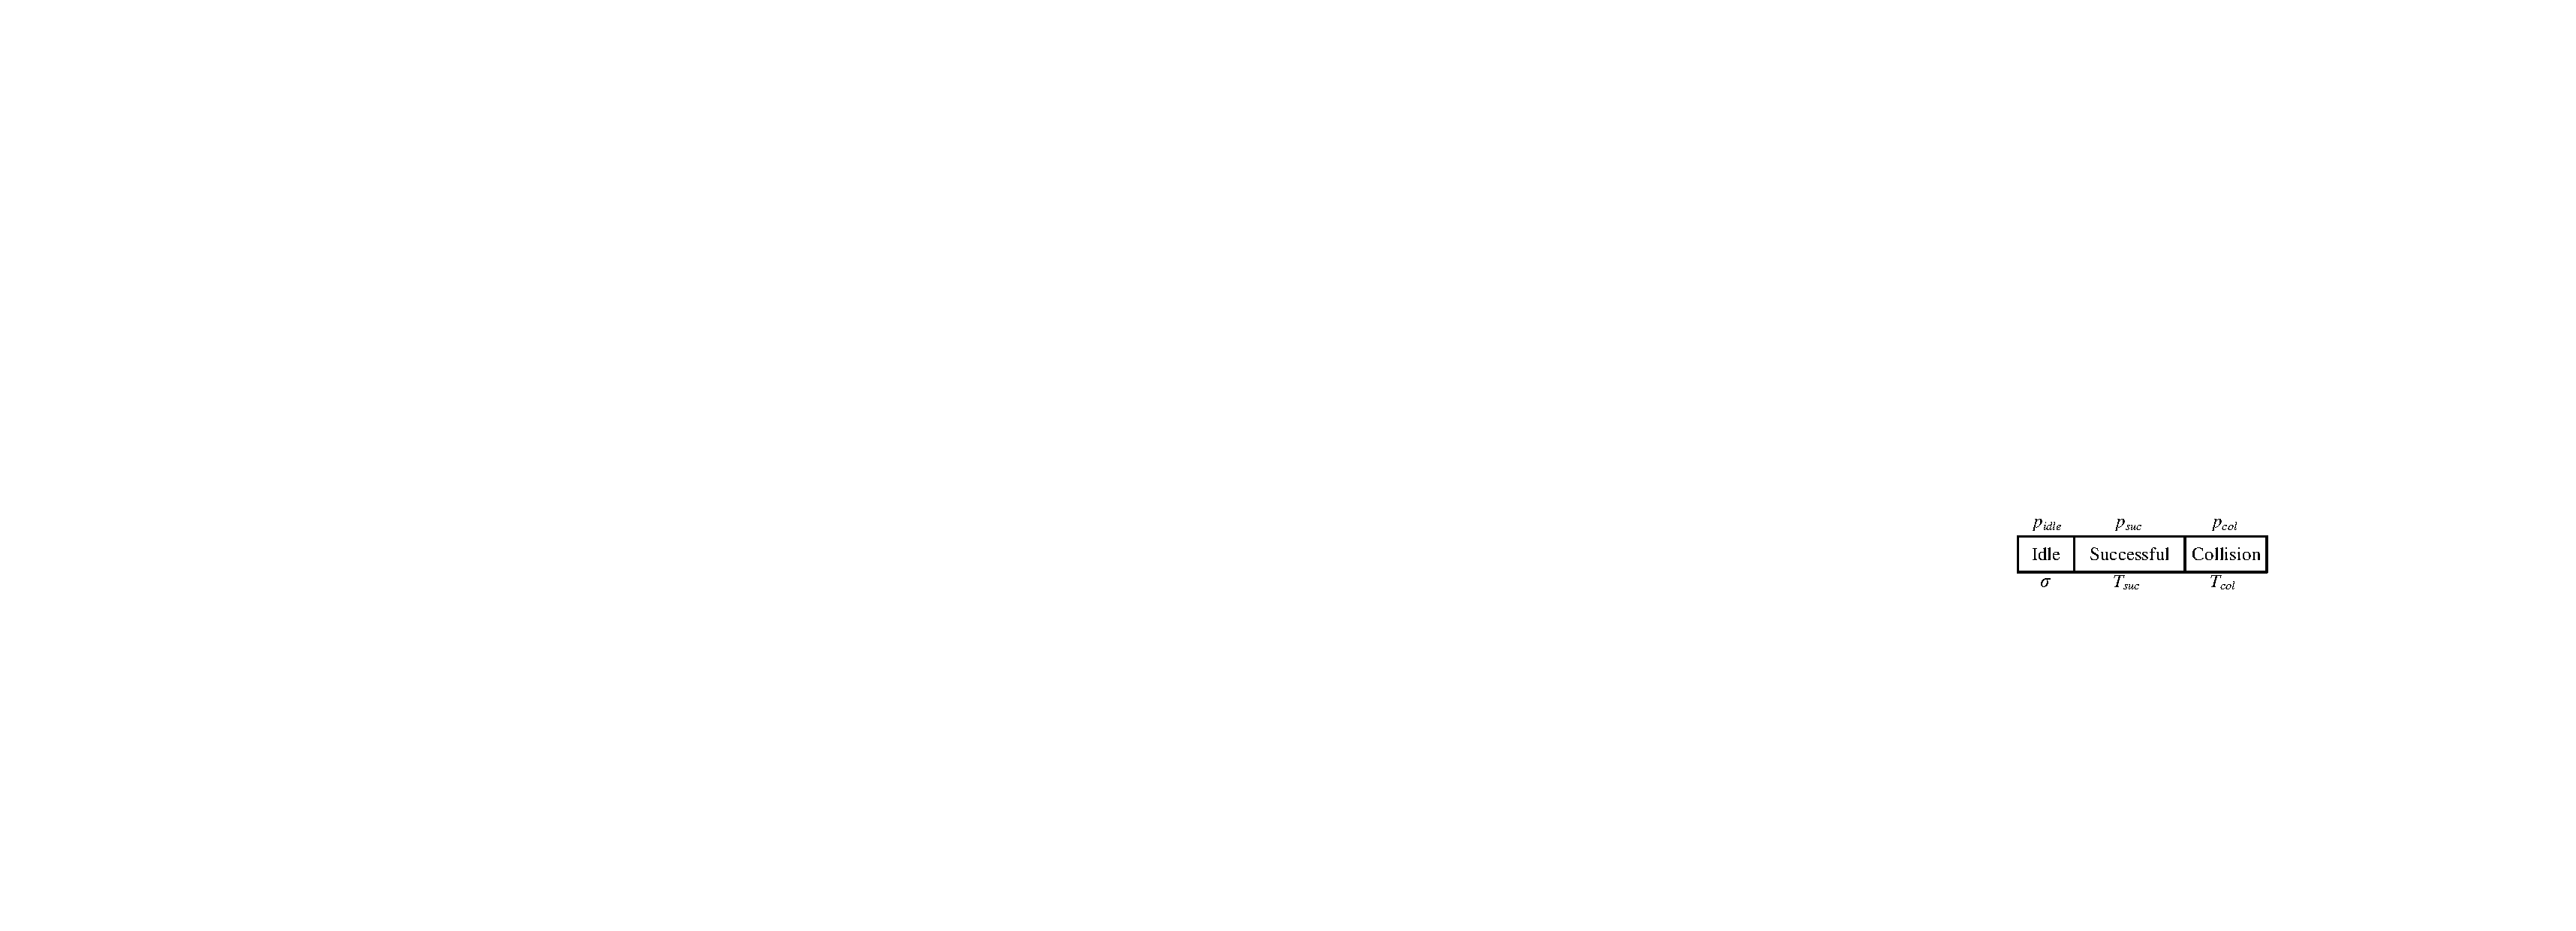
\includegraphics[width=1.75 in]{Figures/virtual_tc.pdf}
 %     \caption{Virtual transmission cycle.}
 %     \label{virtual_tc}
 % \end{figure}

 % \begin{figure*}[htp]
 %     \centering    
 %     
\includegraphics[width=5 in]{Figures/FPTU_logo.png}
 %     \caption{Large figure.}
 %     \label{large_fig}
 % \end{figure*}

 %  Figure \ref{virtual_tc} illustrates the virtual transmission cycle...

% ---- Mathematics ---- 

 % The equation $E=mc^2$ is discovered in 1905 by Albert Einstein. \\
 % The transmission probability
 % \begin{equation}
 %     \tau_{e}=\left[ \frac{1-q_{e}}{q_{e}} \right]
 %     \label{tau_e}
 % \end{equation}

 % According to $\tau_{e}=\left[ \frac{1-q_{e}}{q_{e}} \right]$

% ---- Algorithm ---- 

% \begin{algorithm}
%  	\caption{An algorithm with caption}\label{alg:two}
%  	\begin{algorithmic}
%  		\STATE $i\gets 10$
%  		\IF {$i\geq 5$} 
%  		\STATE $i\gets i-1$
%  		\ELSE
%  		\IF {$i\leq 3$}
%  		\STATE $i\gets i+2$
%  		\ENDIF
%  		\ENDIF 
%  	\end{algorithmic}
%  \end{algorithm}

 % \section{Simulation}
 % \label{sim_sec}

% ---- Citation ---- IEEE/APA

 % The HER-MAC \cite{dang2014her,saxena2021gender} allows vehicle nodes to send safety messages without collision on the Control Channel (CCH) within their reserved time slots and to utilize the SCH resources during the control channel interval (CCHI) for the non-safety message transmissions. Other existing proposals \cite{Wu_WireNet_2016,Huang_WCSP_2020} ...
 % \cite{li2018deepsign} and new paper \cite{saxena2021gender}
 
\section{Conclusion}

% The paper proposes the UR-MAC protocol which allows stations to register uplink communication in advance. The AP assigns RAW slots to the uplink registered stations. It results in the number of transmitting stations in each RAW slot approaching the average number of transmitting stations. The maximum number of successful uplink data packets is close to the average number of successful uplink data packets. The UR-MAC protocol improves the fairness index among stations compared to the IEEE 802.11ah. 

 \bibliographystyle{IEEEtran}  % IEEE
 \bibliography{Mybib}          % IEEE

% \printbibliography{}           % APA

\end{document}